% ==========================================
% فایل: steps/step04.tex
% گام ۴: محاسبه ماتریس هموگرافی و بازیابی
% ==========================================

\section{گام (۴): محاسبه ماتریس هموگرافی و انتقال دستگاه مختصات}

\begin{stepbox}
\field{روند کار و حذف داده‌های پرت با \lr{RANSAC}}{
در گام قبلی دیدیم که تطابق‌ها دارای درصدی خطا (\lr{Outliers}) هستند. اگر تمام این نقاط مستقیماً وارد محاسبات شوند، ماتریس انتقال ۳ در ۳ هندسی (\lr{Homography Matrix}) به شدت دچار اعوجاج می‌شود. برای حل این مشکل، از الگوریتم \lr{RANSAC} استفاده کردیم. این الگوریتم به صورت تکرارشونده، زیرمجموعه‌های تصادفی از نقاط را انتخاب کرده و ماتریسی را می‌سازد که بیشترین توافق (\lr{Inliers}) را با مدل هندسی داشته باشد و داده‌های پرت را نادیده بگیرد.
}

\begin{codebox}[یافتن ماتریس هموگرافی مقاوم]
\begin{lstlisting}[language=Python]
# 1. Extract (x, y) coordinates of the matched keypoints
src_pts = np.float32([kp2_sift[m.trainIdx].pt for m in good_matches]).reshape(-1, 1, 2)
dst_pts = np.float32([kp1_sift[m.queryIdx].pt for m in good_matches]).reshape(-1, 1, 2)

# 2. Calculate Homography matrix using RANSAC to ignore outliers
# 5.0 is the reprojection error threshold in pixels
H, mask = cv2.findHomography(src_pts, dst_pts, cv2.RANSAC, 5.0)
\end{lstlisting}
\end{codebox}

\field{چالش مختصات منفی و راهکار انتقال (\lr{Translation})}{
یک چالش مهم مهندسی در این گام رخ داد: اگر تصویر دوم در دنیای واقعی در سمت چپ تصویر اول قرار داشته باشد (مانند مجموعه‌ی سوم)، پس از نگاشت با ماتریس هموگرافی، نقاط آن دارای مختصات منفی خواهند شد. تابع \lr{\texttt{warpPerspective}} مختصات منفی را خارج از کادر فرض کرده و تصویر را بی‌رحمانه برش می‌دهد (\lr{Cropping}).
برای رفع این مشکل، با محاسبه‌ی کمترین مقدار منفیِ نقاط در فضای جدید، یک ماتریس جابه‌جایی (\lr{Translation Matrix}) به نام $H_t$ تشکیل دادیم. این ماتریس کل بوم نقاشی را به سمت مقادیر مثبت شیفت می‌دهد تا هیچ پیکسلی از بین نرود.
}

\begin{codebox}[جلوگیری از برش با اعمال شیفت هندسی]
\begin{lstlisting}[language=Python]
# 1. Find the minimum x and y coordinates after perspective transform
[xmin, ymin] = np.int32(all_corners.min(axis=0).ravel() - 0.5)
[xmax, ymax] = np.int32(all_corners.max(axis=0).ravel() + 0.5)

# 2. Create a translation matrix to shift negative coordinates to positive domain
t = [-xmin, -ymin]
Ht = np.array([[1, 0, t[0]], [0, 1, t[1]], [0, 0, 1]])

# 3. Calculate new expanded canvas size
canvas_w = xmax - xmin
canvas_h = ymax - ymin

# 4. Warp the image using the combined transformation (Translation * Homography)
img2_warped = cv2.warpPerspective(img2_rgb, Ht.dot(H), (canvas_w, canvas_h))
\end{lstlisting}
\end{codebox}

\field{تحلیل بصری تصاویر بازیابی شده (\lr{Warped Images})}{
تصاویر خروجی به وضوح نشان می‌دهند که زاویه‌ی دیدِ تصویر دوم دچار چرخش و کِش‌آمدگی شده است تا کاملاً با پرسپکتیو تصویر اول هم‌راستا شود. نواحی سیاه‌رنگ در اطراف این تصاویر، نشان‌دهنده‌ی مختصاتی است که خارج از میدان دید دوربینِ دوم بوده و هیچ اطلاعات رنگی برای آن‌ها ثبت نشده است. این نواحی تاریک پس از ترکیب با تصویر اصلی در گام نهایی، به طور کامل پوشش داده می‌شوند.
}
\end{stepbox}

\begin{figure}[h!]
    \centering
    \begin{subfigure}{0.48\textwidth}
        \centering
        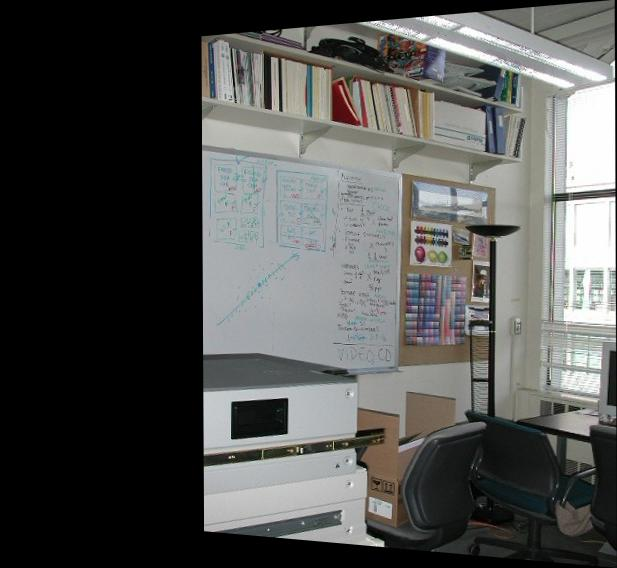
\includegraphics[width=\textwidth]{images/Part_4/Warped_View2_set1.jpg}
        \caption{مجموعه اول: کِش‌آمدگی لبه‌ها برای تطبیق پرسپکتیو}
    \end{subfigure}
    \hfill
    \begin{subfigure}{0.48\textwidth}
        \centering
        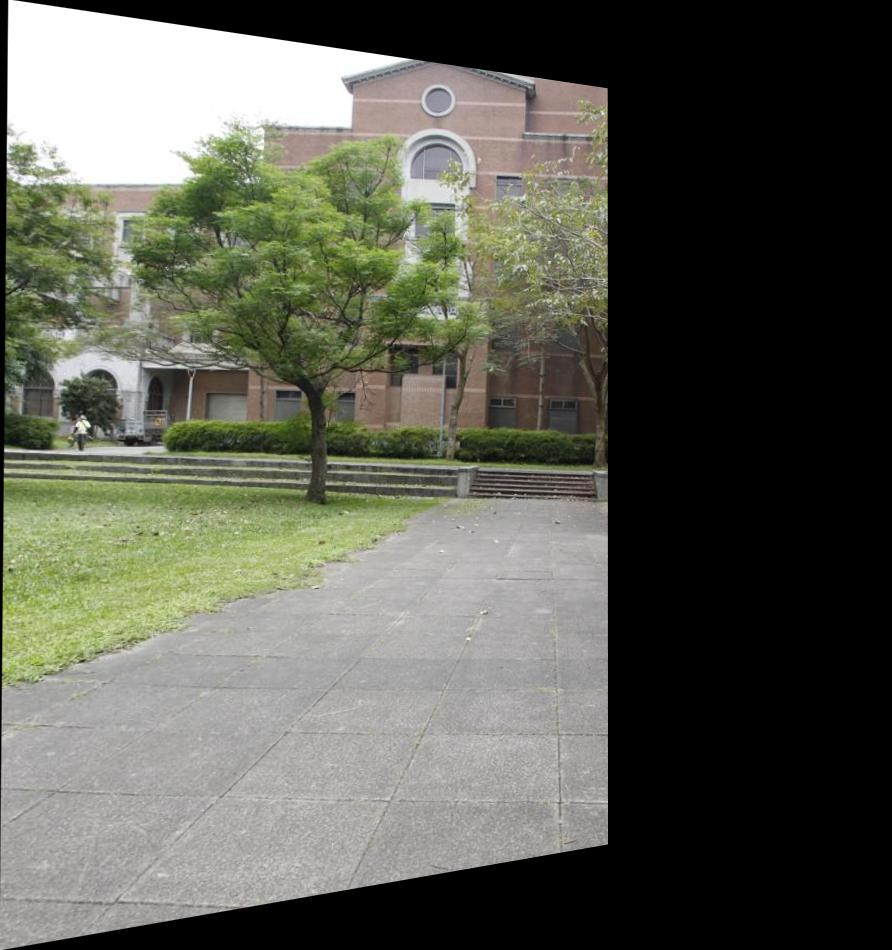
\includegraphics[width=\textwidth]{images/Part_4/Warped_View2_set2.jpg}
        \caption{مجموعه دوم: اعمال هموگرافی روی نمای ساختمان}
    \end{subfigure}
    
    \vspace{0.4cm}
    \begin{subfigure}{0.6\textwidth}
        \centering
        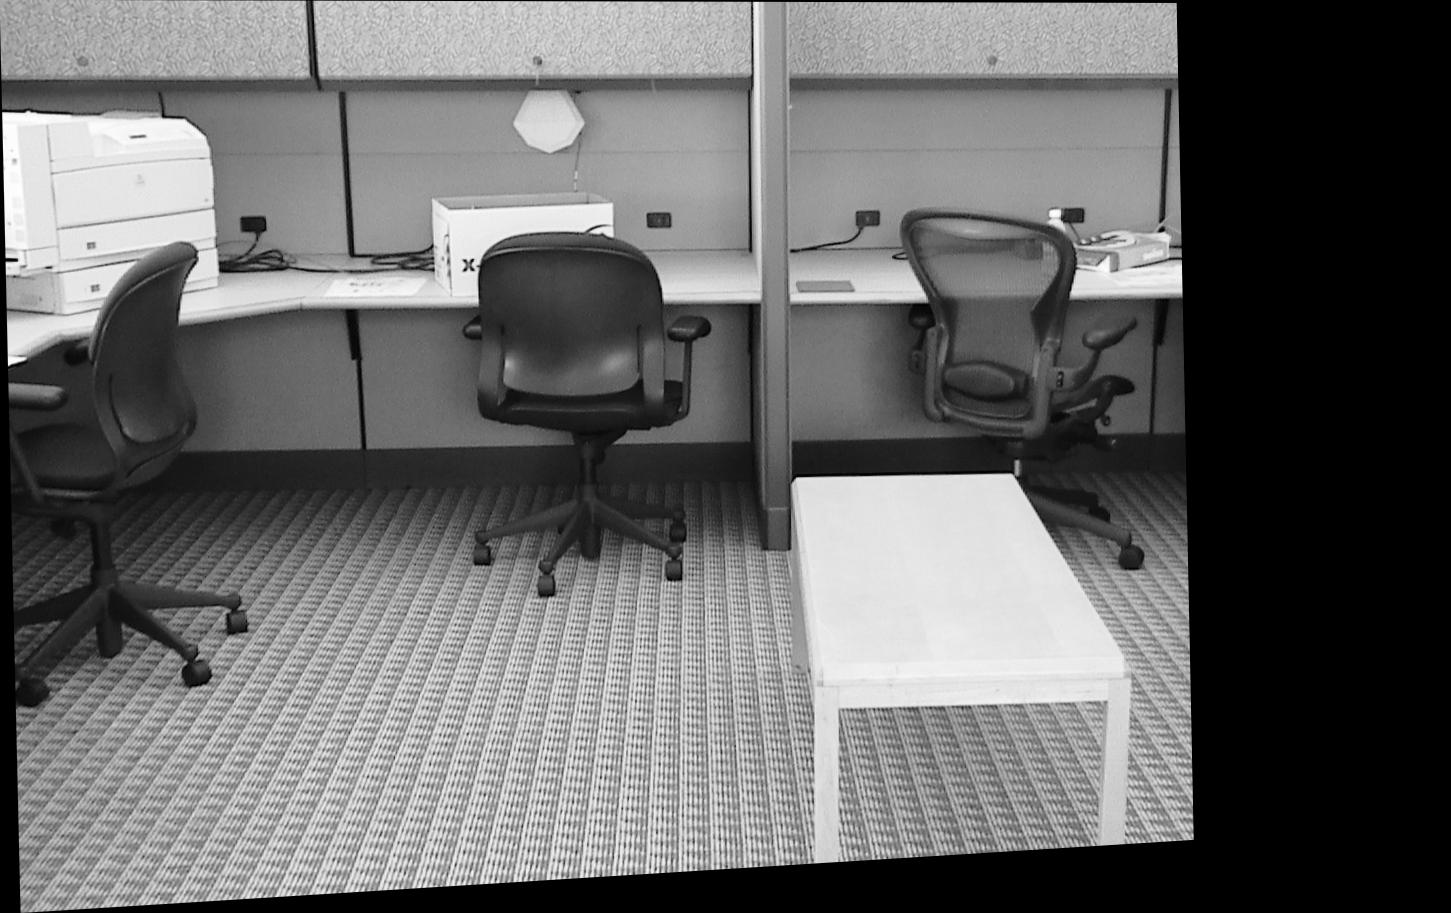
\includegraphics[width=\textwidth]{images/Part_4/Warped_View2_set3.jpg}
        \caption{مجموعه سوم: شیفت موفقیت‌آمیز تصویر به راست برای جلوگیری از برش}
    \end{subfigure}
    \caption{تصاویر بازیابی‌شده (\lr{Warped}) پس از اعمال ماتریس‌های هموگرافی و انتقال}
\end{figure}